\documentclass[openany]{article}
\usepackage[a4paper,margin=1in,bottom=1.5in]{geometry} % define margins. Bottom margin is used to lift a little bit the page number.
\usepackage[english]{babel} % document language is english
\usepackage{tikz} % for drawing (currently not used).
\usepackage{graphicx} % for including images
\usepackage[export]{adjustbox}
\usepackage{fancyhdr} % used for creating headers and footers. only used in title page in this document.
\usepackage{tabularx} % creation of more complex tables
\usepackage{longtable} % tables can span multiple pages
\usepackage{array} % allow elements of tabular environment to have vertical alignment, e.g., center alignment.
\usepackage{nameref} % make it possible to reference by name
\usepackage{hyperref} % allow hiperlinks (links to other document parts and extern links)
\usepackage{etoc} % used for generation of section local table of contents
\usepackage{placeins} % defines the \FloatBarrier command
\usepackage{siunitx} % SI units package
\usepackage{xcolor} % for modifying box color
\usepackage{adjustbox} % for modifying box parameters

% Define graphics path
\graphicspath{{figs/}}

% Configure the cross reference hyper links color
\hypersetup{
    colorlinks=true,
    linkcolor=blue,
}

\newcolumntype{C}{>{\centering\arraybackslash}X} % new column type for tabularx
						 % centered (\centering), adjust width in order to fill table width (X type)

% Configure header in 'titlepage'
\pagestyle{fancy}
\lhead{\includegraphics[width=4.5cm]{logo_cnpem}}
\rhead{\includegraphics[width=4cm]{logo_lnls}}
\renewcommand{\headrulewidth}{0pt}
\setlength{\headheight}{52pt}
% Clean footer
\fancyfoot{}

% increase table height factor a little bit (taller cells)
\renewcommand{\arraystretch}{1.5}

%==== Begin DOCUMENT ====
\begin{document}

%--- Begin title page ---
\begin{titlepage}

% Add header to this page
\thispagestyle{fancy}

% Center elements
\begin{center}

% title of title page
\topskip0pt % perfectly centered
\vspace*{\fill}
\textbf{\Huge DCCT EPICS Application User Guide}\\[20pt]
\textbf{\Huge Version 3.0}\\[20pt]
\textbf{\Huge September/2024}
\vspace*{\fill}

% footer of title page
\vfill
\textbf{Brazilian Synchrotron Light Laboratory (LNLS)}\\[5pt]
\textbf{Brazilian Center for Research in Energy and Materials (CNPEM)}
\end{center}

\end{titlepage}
%--- End of title page ---

\newpage
\pagestyle{plain} % restore default page style

%--- About this manual ---
\paragraph{}{\Large\bfseries About this manual}

\paragraph{} This manual provides an overview of the DCCT EPICS application. It is assumed that the reader is familiar with the basics of EPICS.

%--- Table of contents ---
\tableofcontents

\newpage
%--- Section: Introduction ---
\section{Introduction}

\paragraph{} The Direct-Current Current Transformer (DCCT) is the sensor responsible for measuring the beam average current. The DCCT application software is responsible for making DCCT measurements and configuration options available as EPICS Process Variables (PVs).

%--- Section: Instrument Setup ---
\section{Instrument Setup}
\subsection{Common Instrument Setup}

	\paragraph{} The complete DCCT measurement setup consists of a DCCT (Bergoz NPCT) mounted in the beam line; a digital multimeter (Kethley DMM7510) connected to the DCCT output terminals; a STD-EVE timing module, which has a multimeter trigger output connected to its rear panel and one of its front panel outputs connected to the multimeter trigger input; a PC which communicates with the digital multimeter; a connection to a remote module from the interlock system for DCCTs in the Storage Ring.

	% Instrument Setup figure
	\begin{figure}[!h]
		\caption{Instrument Setup}
		\label{fig:dcct-setup}
		\centering
		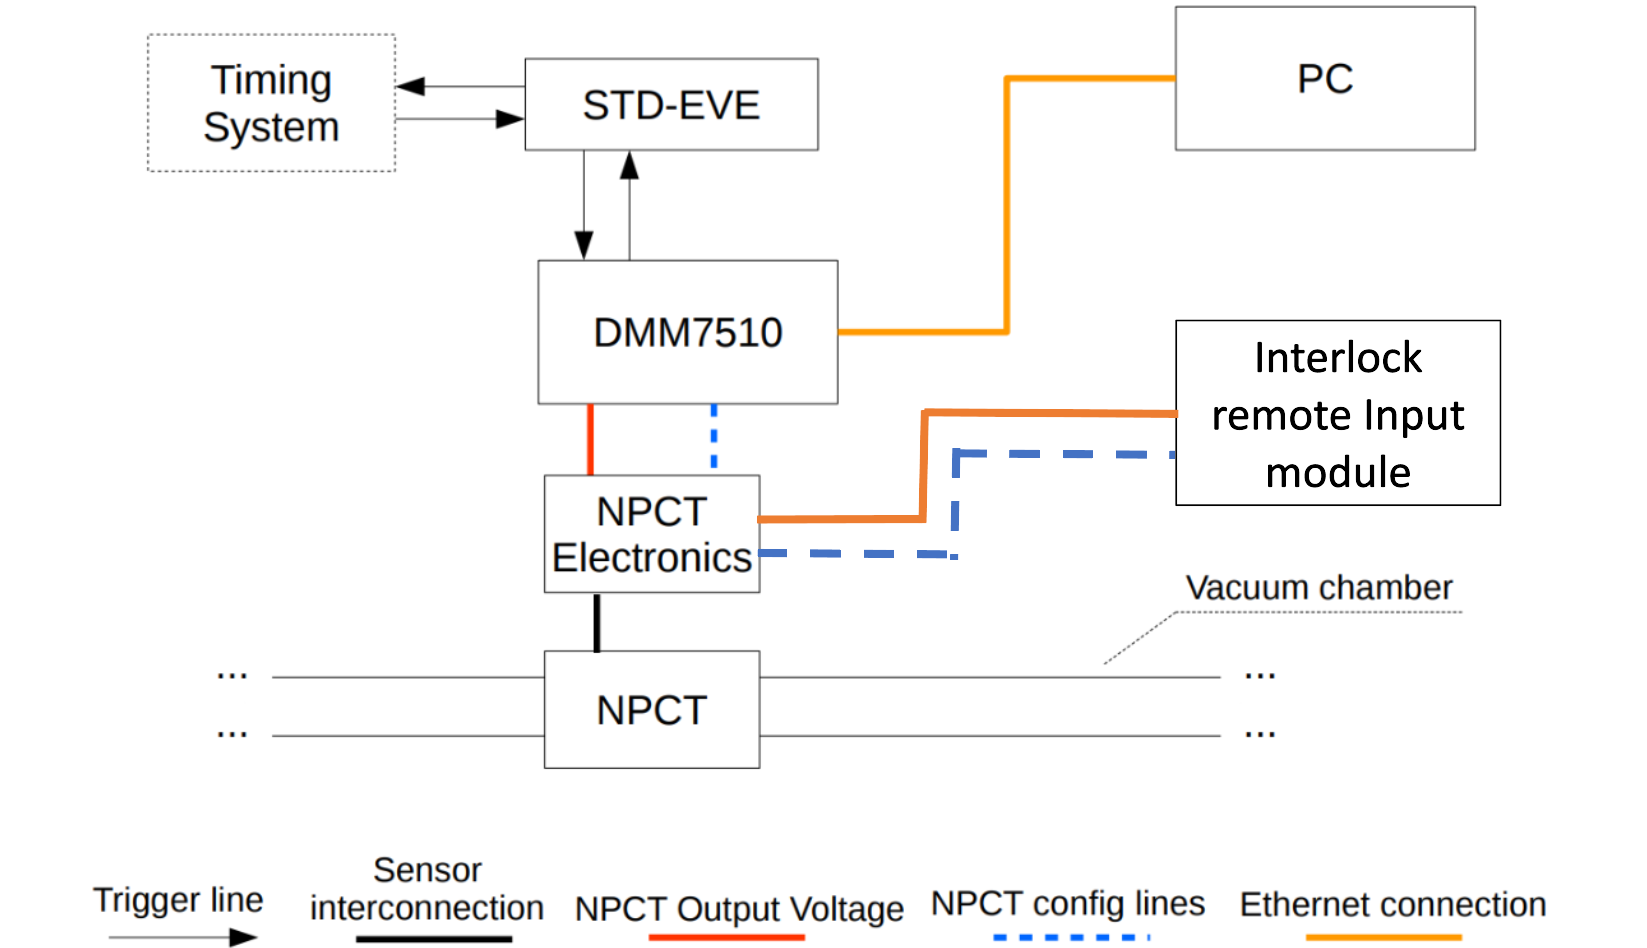
\includegraphics[width=1.0\textwidth]{dcct_interlock_14c4}
	\end{figure}
\FloatBarrier

	\paragraph{} The NPCT (New Parametric Current Transformer) is a comercial DCCT, fabricated by Bergoz Instrumentation, widely used in particles accelerators around the world for measuring average beam current. The instrument generates a voltage output, in the 0 to 10 volts range, proportional to the current flowing through its toroid.

	\paragraph{} The Kethley DMM7510 digital multimeter is connected to the NPCT voltage output and is used to acquire, convert, and filter the sensor data. For the Storage Ring DCCT, the multimeter is also responsible for generating a trigger to the STD-EVE timing module whenever the current falls below a specified threshold, indicating that the beam has been lost.

	\paragraph{} The STD-EVE timing module can trigger multimeter readings, and monitor the multimeter output trigger line. Upon trigger reception, the STD-EVE generates a post-mortem event that is broadcast to the entire Timing System.

	\paragraph{} The PC runs an EPICS IOC, which includes DMM7510 multimeter and DCCT application-specific PVs. The application reads the multimeter data regularly and configures the multimeter's parameters according to the settings defined in the application PVs.

 	\paragraph{} The connection to the interlock system consists of 2 signals for the sensor in the sector 14C4 of the Storage Ring. A monitor signal for the interlock to read the current NPCT electronics range configuration, which is defined by the DMM7510 multimeter, and a copy of the NPCT measurement output signal, provided on the front panel of the electronics. For the sensor at the sector 13C4, which is considered by the interlock system as the the most reliable source of current reading, only the DCCT measurement output signal is provided, since the NPCT range is fixed for greater safety. The DCCT in the Booster is not connected to the interlock system. More details are provided in \emph{\nameref{sec:integration-interlock}}.

\subsection{DCCT Integration to Interlock}\label{sec:integration-interlock}

	\paragraph{} The Sirius personal protection system uses the DCCT measurement as one of the variables to determine if there is an electron beam inside of the accelerator tunnel. The presence of beam is used in the interlock logic for personal protection. To minimize the number of points of failure in the measurement process for interlock, the interlock system bypasses the digital multimeter and is connected directly to the NPCT electronics instead. The NPCT electronics has an additional signal output on the front panel (besides the main signal output on the back). This front output is connected to an analog input channel of a remote input/output module which is located in the same rack as the NPCT electronics. The interlock system converts the analog reading from the NPCT output to a current measurement value. For greater safety, the range of the NPCT corresponding to the DCCT in sector 13C4 of the Storage Ring is fixed by hardware by means of a jumper connected to the NPCT electronics configuration input connector. The software can be configured through the device option during deploy to disable range configuration so that the digital multimeter and the NPCT electronics are always consistency regarding the measurement range. This guarantees that the reading displayed in the control room and archived is consistent to the measured value. The interlock system is not impacted by the software readings, since the multimeter is bypassed for the interlock.

	% Instrument Setup figure
	\begin{figure}[!h]
		\caption{DCCT integration to the Interlock system for sensor at sector SI-13C4}
		\label{fig:dcct-special-setup}
		\centering
		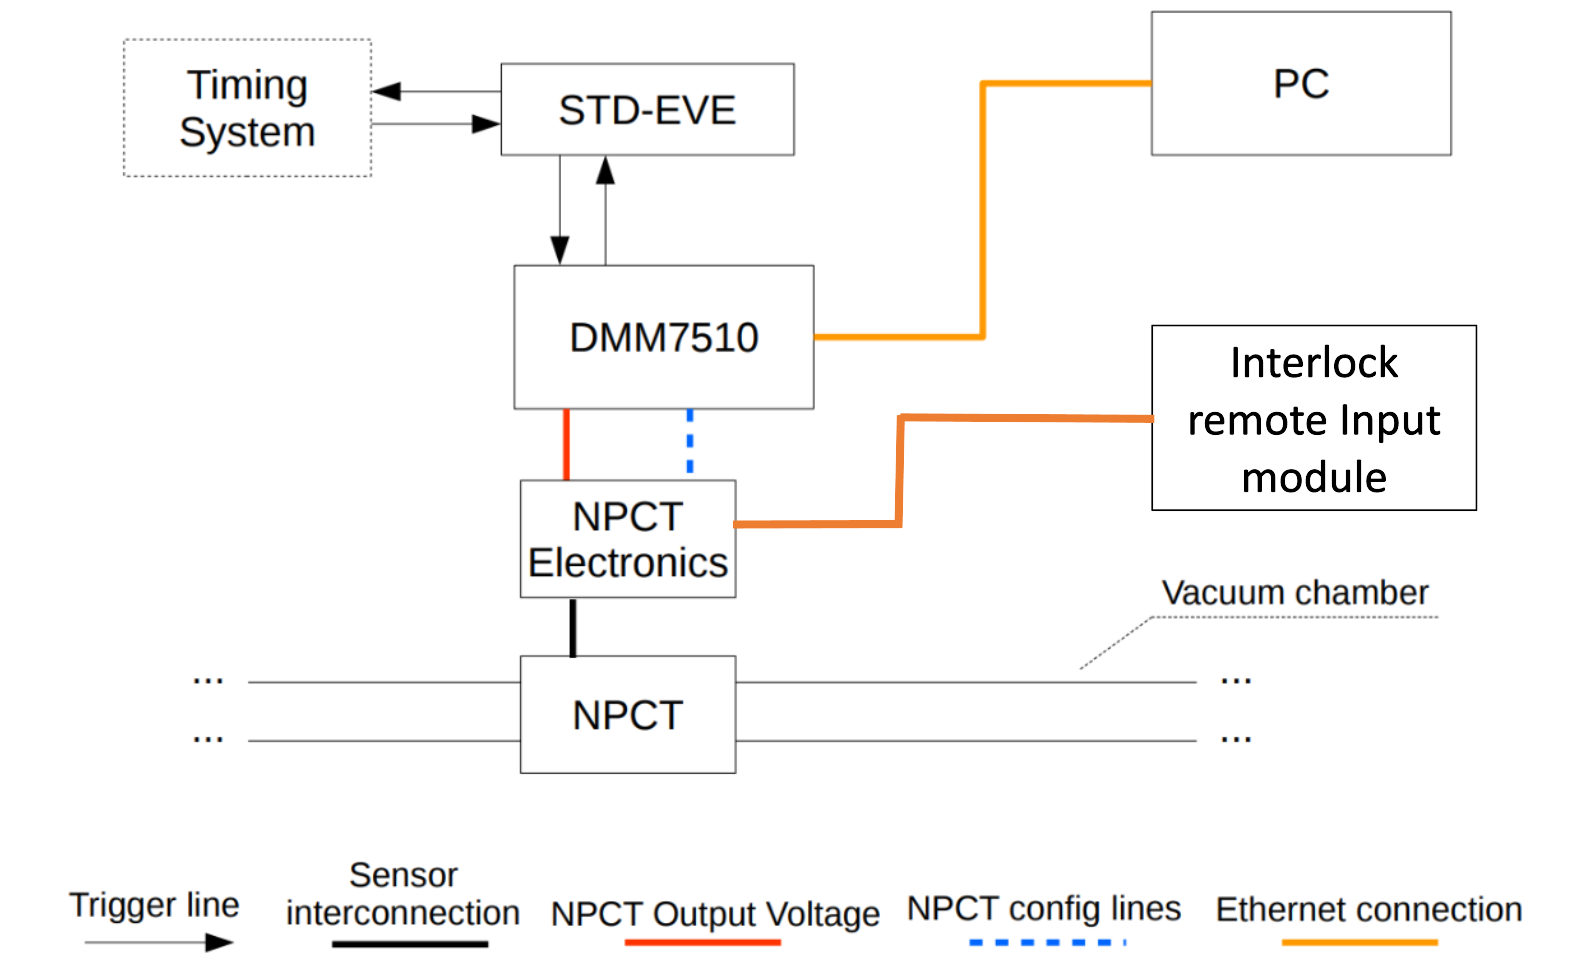
\includegraphics[width=1.0\textwidth]{dcct_interlock_13c4}
	\end{figure}
\FloatBarrier

%--- Section: Measurement Overview ---
\section{Measurement Overview}

	\subsection{Storage Ring} 

		\paragraph{} Storage Ring beam current is measured periodically in fixed time steps. The measurement trigger can be provided by software or by an external trigger pulse. When software triggering is selected, the DCCT application issues measurement commands at a "as fast as possible" rate, which is constrained by the measurement duration. Therefore, the software triggering rate is defined by the measurement period plus some latency, up to 50 Hz. When external triggering is selected, the multimeter starts a measurement once an external trigger is received from the Timing System. The IOC monitoring rate and data transfer latency limit the effective measurement rate, which cannot be as fast with external triggering as with software triggering.

		\paragraph{} Another important task of the Storage Ring DCCT system is to inform the Timing System whenever the beam current falls below a minimum threshold. If configured to do so, the multimeter constantly monitors the DCCT output while acquisition is enabled, comparing it to the specified threshold. When the current level falls below the threshold, the multimeter outputs a trigger pulse to a STD-EVE timing module in less than \SI{2}{\micro\second}.

	\subsection{Booster} 

		\paragraph{} The Booster beam current measurements must be correlated to each separate Booster ramp cycle, requiring a triggering mechanism. The measurement trigger in this application can be provided by an external trigger pulse or by the beam current level itself. When in external trigger mode, the multimeter measurements are triggered by the STD-EVE module at each Booster ramp cycle. When triggered by current level, a measurement starts when the input signal becomes greater than the specified threshold.

%--- Section: DCCT Software Configuration Steps ---
\section{DCCT Software Configuration}

	\paragraph{} This section describes the basic steps when configuring the DCCT application. Further detail about the DCCT application PVs can be found in \emph{\nameref{sec:process-variables}}.

	\bigskip
	\noindent\adjustbox{minipage=\textwidth,cfbox=red 1.0pt 2ex}{
		It is necessary to \hyperref[acquisition-start]{disable acquisition} before making any changes to the application settings. All of the set point and selection PVs are disabled while the enble status is \emph{ON}. This avoids incorrect measurements, false post-mortem signal generation, temporary communication loss with the multimeter, or even the need to power cycle the multimeter.
	}

	\bigskip
	\noindent\adjustbox{minipage=\textwidth,cfbox=red 1.0pt 2ex}{A new \hyperref[relative-offset]{voltage relative offset} should be acquired every time the range configuration or measurement mode are modified.}

	\bigskip
	\noindent\adjustbox{minipage=\textwidth,cfbox=red 1.0pt 2ex}{When the application is configured for either \emph{External} or \emph{Input-Level-based} triggering, the interval between triggers should be greater than the measurement period by roughly 100 ms. This is necessary to guarantee that the multimeter has enough time to acquire and send the data to the IOC, otherwise triggers issued too soon are ignored.}

	\subsection{Mesurement Mode}\label{measurement-mode}

		\paragraph{Measurement mode selection}\label{measurement-mode-selection} The DMM7510 multimeter can operate in two different acquisition modes, the \emph{Measure} and \emph{Digitize} modes. In the DCCT IOC these modes are referred to as \emph{Normal} and \emph{Fast} modes, respectively. The \emph{Normal} mode provides greater resolution (7 and 1/2 digits, compared to 4 digits for \emph{Fast} mode), while the \emph{Fast} mode can provide slightly higher sample rates and greater resolution (1 more digit than \emph{Normal} mode) for high sample rates (1 Ksamples/s to 1 Msamples/s).

	\bigskip
	\noindent\adjustbox{minipage=\textwidth,cfbox=teal 1.0pt 2ex}{The PVs in the \hyperref[measurement-settings]{Measurement Settings} section are divided in two groups, depending on the type of measurement they are associated with: PVs for the \emph{Normal Mode}, and PVs for the \emph{Fast Mode}.}

			\begin{enumerate}
				\item Set \emph{MeasMode-Sel} PV to the desired mode: \emph{Normal} or \emph{Fast}.
				\item Wait until \emph{MeasMode-Sts} has changed to the chosen option and all the other settings have stabilized in the selected values (this takes a few seconds).
			\end{enumerate}

	\subsection{Measurement triggering}

		\paragraph{Disable triggering}\label{disable-triggering} It might be useful, in some cases, to disable measurement triggering. In this configuration, all trigger types are disabled.

			\begin{enumerate}
				\item Set \emph{MeasTrg-Sel} PV to \emph{None}.
				\item Wait until \emph{MeasTrg-Sts} has changed to \emph{None}.
			\end{enumerate}

		\paragraph{Software triggering} In the software triggering mode, the DMM7510 multimeter starts measurements in response to periodic software requests.

			\begin{enumerate}
				\item Set \emph{MeasTrg-Sel} PV to \emph{Software}.
				\item Wait until \emph{MeasTrg-Sts} has changed to \emph{Software}.
			\end{enumerate}

		\paragraph{External triggering} In the external triggering mode, the DMM7510 multimeter starts measurements in response to external trigger reception, while software periodically monitors the device to retrieve the newest measurement available.

			\begin{enumerate}
				\item Set \emph{MeasTrg-Sel} PV to \emph{External}.
				\item Wait until \emph{MeasTrg-Sts} has changed to \emph{External}.
			\end{enumerate}

		\paragraph{Input level based triggering} In level based triggering mode, the DMM7510 multimeter starts measurements in response to any beam current rising edge that goes above the specified threshold.

			\begin{enumerate}
				\item Set \emph{Range-Sel} to the desired DCCT sensor range.
				\item Verify if \emph{Range-Sts} has changed accordingly.
				\item Set \emph{CurrThold-SP} to the current level threshold intended to trigger measurements.
				\item Verify if \emph{CurrThold-RB} has changed accordingly.
				\item Set \emph{HFReject-Sel} to indicate if high frequency rejection should be used.
				\item Verify if \emph{HFReject-Sts} has changed accordingly.
				\item Set \emph{MeasTrg-Sel} to \emph{InLevel}.
				\item Wait until \emph{MeasTrg-Sts} has changed to \emph{InLevel}.
			\end{enumerate}

	\subsection{DCCT Range selection}

		\paragraph{} The selected DCCT sensor range should never be smaller than the current passing through the sensor. Currents exceeding the full scale range may saturate the sensor magnetic cores. In order to desaturate it, power cycle the NPCT electronics.

			\begin{enumerate}
				\item Set \emph{Range-Sel} to the desired DCCT sensor range.
				\item Verify if \emph{Range-Sts} has changed accordingly.
			\end{enumerate}

	\subsection{Low beam current detection}

		\paragraph{} Low beam current detection is used for post-mortem signal generation. \emph{This feature cannot be used along with input-level-based measurement triggering}.

			\begin{enumerate}
				\item Set \emph{Range-Sel} to the desired DCCT sensor range.
				\item Verify if \emph{Range-Sts} has changed accordingly.
				\item Set \emph{CurrThold-SP} to the desired current level threshold.
				\item Verify if \emph{CurrThold-RB} has changed accordingly.
				\item Set \emph{HFReject-Sel} to indicate if high frequency rejection should be used.
				\item Verify if \emph{HFReject-Sts} has changed accordingly.
				\item Set \emph{LowLimEnbl-Sel} to \emph{ON}.
				\item Verify if \emph{LowLimEnbl-Sts} status is \emph{ON}.
			\end{enumerate}

	\subsection{Measurement settings}\label{measurement-settings}

		% Measurement characteristcs figure 1
		\begin{figure}[!h]
			\caption{Measurement with SampleCnt=3, MeasPeriod=0.6, LineSync=ON}
			\label{fig:meas-param1}
			\centering
			\includegraphics[width=1.0\textwidth]{dcct-meas-param1}
		\end{figure}

		% Measurement characteristcs figure 2
		\begin{figure}[!h]
			\caption{Measurement with SampleCnt=3, MeasPeriod=0.6, AvgFilterEnbl=ON, AvgFilterCnt=5}
			\label{fig:meas-param2}
			\centering
			\includegraphics[width=1.0\textwidth]{dcct-meas-param2}
		\end{figure}
\FloatBarrier

	\bigskip
	\noindent\adjustbox{minipage=\textwidth,cfbox=teal 1.0pt 2ex}{The measurement settings PVs that should be used depend on the selected \hyperref[measurement-mode]{Measurement Mode}. There is an indication above each PV group showing the mode associated to it.}

		\paragraph{General} Some parameters define the measurement sampling characteristics.

			\noindent\adjustbox{cfbox=darkgray 1.0pt 1ex}{Normal Mode PVs}

			\begin{enumerate}
				\item \emph{MeasPeriod-SP} sets the period, in seconds, of a measurement executed in response to a trigger or software request.
				\item \emph{MeasPeriod-RB} indicates the configured measurement period, in seconds.
				\item \emph{SampleCnt-SP} sets the number of samples to be taken during the specified measurement period. The resulting sample aperture is automatically calculated and set.
				\item \emph{SampleCnt-RB} indicates the number of samples taken during each measurement period.
				\item \emph{LineSync-Sel} sets if measurement integration period is synched to power line cycle zero crossing. Line synchronization affects measurement speed. The change in acquisition time caused by this setting is not accounted for by the \emph{MeasPeriod-RB} PV value.
				\item \emph{LineSync-Sts} indicates the configured measurement power line synchronization status.
				\item \emph{Imped-Sel} sets the multimeter's input impedance. Recommended setting is \emph{AUTO}.
				\item \emph{Imped-Sts} indicates the configured multimeter's input impedance.
			\end{enumerate}

			\noindent\adjustbox{cfbox=darkgray 1.0pt 1ex}{Fast Mode PVs}

			\begin{enumerate}
				\item \emph{FastMeasPeriod-SP} sets the period, in seconds, of a measurement executed in response to a trigger or software request.
				\item \emph{FastMeasPeriod-RB} indicates the configured measurement period, in seconds.
				\item \emph{FastSampleCnt-SP} sets the number of samples to be taken during the specified measurement period. The resulting sample aperture is automatically calculated and set.
				\item \emph{FastSampleCnt-RB} indicates the number of samples taken during each measurement period.
				\item \emph{FastImped-Sel} sets the multimeter's input impedance. Recommended setting is \emph{AUTO}.
				\item \emph{FastImped-Sts} indicates the configured multimeter's input impedance.
			\end{enumerate}

		\paragraph{Filter} It is possible to apply an averaging filter to measurements. If enabled, the specified number of samples are taken and averaged by the specified algorithm.

			\noindent\adjustbox{cfbox=darkgray 1.0pt 1ex}{Normal Mode PVs}

			\begin{enumerate}
				\item \emph{AvgFilterCnt-SP} sets the number of measurements that are used to produce a reading. The change in acquisition time caused by this setting is not accounted for by the \emph{MeasPeriod-RB} PV value.
				\item \emph{AvgFilterCnt-RB} indicates the configured number of measurements used to produce a reading.
				\item \emph{AvgFilterTyp-Sel} sets the average filter algorithm used. The \emph{Repeat} algorithm affects the acquisition time, while the \emph{Moving average} algorithm does not.
				\item \emph{AvgFilterTyp-Sts} indicates the configured average filter algorithm.
				\item \emph{AvgFilterWind-SP} sets the average filter window. When a filter sample value exceeds the window threshold, the filter stack is filled immediately with that sample value.
				\item \emph{AvgFilterWind-RB} indicates the filter configured window.
				\item \emph{AvgFilterEnbl-Sel} enables/disables filtering.
				\item \emph{AvgFilterEnbl-Sts} indicates the filter enable status.
			\end{enumerate}

	\bigskip
	\noindent\adjustbox{minipage=\textwidth,cfbox=darkgray 1.0pt 2ex}{There are no filter settings for the \emph{Fast} measurement mode.}

		\paragraph{Relative offset}\label{relative-offset} The relative offset parameter is used to remove offsets caused by instrument zero drift.

			\noindent\adjustbox{cfbox=darkgray 1.0pt 1ex}{Normal Mode PVs}

			\begin{enumerate}
				\item \emph{RelLvl-SP} sets the relative offset voltage level. The offset is subtracted from the measured voltage before any conversion is performed.
				\item \emph{RelLvl-RB} indicates the configured relative offset voltage level.
				\item \emph{RelEnbl-Sel} enables/disables the relative offset.
				\item \emph{RelEnbl-Sts} indicates the relative offset enable status.
				\item \emph{RelAcq-Cmd} sets the relative offset level equal to the multimeter input voltage level.
			\end{enumerate}

			\noindent\adjustbox{cfbox=darkgray 1.0pt 1ex}{Fast Mode PVs}

			\begin{enumerate}
				\item \emph{FastRelLvl-SP} sets the relative offset voltage level. The offset is subtracted from the measured voltage before any conversion is performed.
				\item \emph{FastRelLvl-RB} indicates the configured relative offset voltage level.
				\item \emph{FastRelEnbl-Sel} enables/disables the relative offset.
				\item \emph{FastRelEnbl-Sts} indicates the relative offset enable status.
				\item \emph{FastRelAcq-Cmd} sets the relative offset level equal to the multimeter input voltage level.
			\end{enumerate}

	\subsection{Stored Beam Status Configuration}

		\paragraph{} The IOC provides a PV which indicates when there is stored beam. This is done by comparing the current measurement with an user-configurable threshold.

		\begin{enumerate}
			\item Set \emph{CurrThold-SP} to the desired current level threshold, if not already configured.
			\item Verify if \emph{CurrThold-RB} is configured accordingly.
			\item \emph{StoredEBeam-Mon} indicates if the current is above the configured threshold, meaning that there is stored beam.
		\end{enumerate}

	\subsection{Acquisition Start}\label{acquisition-start}

		\paragraph{} The acquisition needs to be enabled for the instrument to start monitoring current. The acquisition can only start when valid configuration options have been selected.

	\bigskip
	\noindent\adjustbox{minipage=\textwidth,cfbox=red 1.0pt 2ex}{While acquisition is enabled, NO change is allowed to the DCCT settings. Any command apart from \emph{acquisition disable} and \emph{download} are ignored.}

	\bigskip
	\noindent\adjustbox{minipage=\textwidth,cfbox=teal 1.0pt 2ex}{It is recommended that, after enabling acquisition, the user checks if the measurements are updating at the intended rate. The information is provided by the \emph{MeasUpdatePeriod-Mon} PV. When measurement update rate is slower than desired, the solution may be to reduce the number of samples per measurement (\emph{SampleCnt-SP}) or the measurement period (\emph{MeasPeriod-SP}). If you are using external triggering, check if the external trigger source is correctly configured. Also, make sure that the \emph{Repeat} filter is disabled, and, when using more than 1 sample per measurement, check if the reading is not delayed by line synchronization (\emph{LineSync-Sel}).}

			\begin{enumerate}
				\item \emph{Enbl-Sel} enables/disables the DCCT acquisition and current level monitoring.
				\item \emph{Enbl-Sts} indicates the DCCT acquisition enable status.
			\end{enumerate}

	\subsection{DCCT calibration}

		\paragraph{} The DCCT has a test function which injects a +100mA test signal in the sensor head when enabled.

			\begin{enumerate}
				\item \emph{Test-Sel} enables/disables the DCCT calibration current.
				\item \emph{Test-Sts} indicates the DCCT calibration current enable status.
			\end{enumerate}

	\subsection{Save function}

		\paragraph{} The EPICS autosave module periodically saves the current PV values and restore them when the IOC is restarted.

%--- Section: Reading Measurements from PVs ---
\section{Reading Measurements from PVs}

	\paragraph{} The DCCT measurement data is available in the following EPICS PVs.

		\begin{enumerate}
			\item \emph{RawReadings-Mon} stores the last measurement waveform acquired.
			\item \emph{Current-Mon} stores the average of the last waveform acquired, which represents the latest measurement.
			\item \emph{CurrHstr-Mon} is a circular buffer storing the last 1000 measurements from \emph{Current-Mon}.
			\item \emph{Timestamp-Mon} stores the timestamp from \emph{Current-Mon} as a double representation of UTC in seconds and subseconds since 1 January 1970.
			\item \emph{TimestampHstr-Mon} is a circular buffer storing the last 1000 values from \emph{Timestamp-Mon}.
			\item \emph{ClearHstr-Cmd} clears both \emph{CurrHstr-Mon} and \emph{TimestampHstr-Mon} circular buffers, when set to 1. This command is useful when there are old or invalid values in the history that should be discarded before some high level task is executed.
			\item \emph{ReliableMeas-Mon} indicates if the DCCT application measurements at each instant are reliable. This PV is an \emph{OR} of the \emph{temperature calibration warning}, \emph{network disconnect status} and \emph{acquisition disabled status}. If any of these conditions are true, a measurement update is not considered to be reliable.
		\end{enumerate}

\newpage
\section{Process Variables Description}\label{sec:process-variables}

	% Process Variables description table
	\begin{longtable}{| m{3.0cm} m{4.5cm} m{7.0cm} |}
		\caption{Application Process Variables} \\ \hline
		\bfseries Name & \bfseries Data Type & \bfseries Description \label{tab:PV-description} \endfirsthead
		\caption{Application Process Variables} \\ \hline
		\bfseries Name & \bfseries Data Type & \bfseries Description \endhead \hline
		% --- row ---
		Enbl-Sel & BOOL: OFF, ON & \begin{tabular}{@{}m{6cm}@{}}
	    					Acquisition enable. This PV starts acquisition when set to \emph{ON} (1). When the selected instrument configuration is invalid, this PV is forced back to \emph{OFF}. This PV enables not only acquisition, but also low current level detection, when it is configured. While acquisition is enabled, the only PVs that accept changes are \emph{Enbl-Sel} itself and \emph{Download-Cmd}.
						\end{tabular} \\ \hline
		% --- row ---
		Enbl-Sts & ENUM: OFF, ON, PREPARING & \begin{tabular}{@{}m{6cm}@{}}
	    					Acquisition enable status. This PV indicates the acquisition status. When \emph{PREPARING} is displayed, the IOC is configuring the instrument to start acquisition. When the enable status is \emph{ON}, acquisition has started and \emph{NO change to DCCT settings is allowed}.
						\end{tabular} \\ \hline
		% --- row ---
		MeasMode-Sel & ENUM: Normal, Fast & \begin{tabular}{@{}m{6cm}@{}}
	    					Measurement acquisition mode. This PV selects the acquisition mode used by the multimeter, which can be 'Normal' or 'Fast'. When using 'Fast' acquisition, higher sample rates (1 KHz to 1 MHz) have greater resolution when compared to the 'Normal' mode. On the other hand, 'Normal' acquisition provides the best resolution as long as the sample period is long enough. Some PVs are specific to a given measurement mode and, when this is the case, this will be indicated at the PV description.
						\end{tabular} \\ \hline
		% --- row ---
		MeasMode-Sts & ENUM: Unknown, Normal, Fast & \begin{tabular}{@{}m{6cm}@{}}
	    					Measurement acquisition mode status. When the multimeter function is misconfigured, this PV displays the 'Unknown' status.
						\end{tabular} \\ \hline
		% --- row ---
		Current-Mon & FLOAT: 32-bit & \begin{tabular}{@{}m{6cm}@{}}
	    					Latest current measurement. This PV holds the average of the latest measurement waveform fetched from the multimeter.
						\end{tabular} \\ \hline
		% --- row ---
		CurrHstr-Mon & FLOAT[1000] & \begin{tabular}{@{}m{6cm}@{}}
	    					Current measurement history. This PV is a circular buffer holding the last 1000 values of the PV \emph{Current-Mon}.
						\end{tabular} \\ \hline
		% --- row ---
		RawReadings-Mon & FLOAT[1000000] & \begin{tabular}{@{}m{6cm}@{}}
	    					Latest measurement raw waveform. This PV holds the last waveform fetched from the multimeter. The waveform count is defined by the \emph{SampleCnt-SP} PV for \emph{Normal} acquisition, and by the \emph{FastSampleCnt-SP} PV for \emph{Fast} acquisition.
						\end{tabular} \\ \hline
		% --- row ---
		Timestamp-Mon & FLOAT: 32-bit & \begin{tabular}{@{}m{6cm}@{}}
	    					Timestamp of latest current measurement. This PV holds the timestamp of the latest update of the \emph{Current-Mon} PV. The timestamp is a floating point representing UTC as the seconds and subseconds since 1 January 1970.
						\end{tabular} \\ \hline
		% --- row ---
		TimestampHstr-Mon & FLOAT[1000] & \begin{tabular}{@{}m{6cm}@{}}
	    					Timestamp history. This PV is a circular buffer holding the last 100 values of the PV \emph{Timestamp-Mon}.
						\end{tabular} \\ \hline
		% --- row ---
		ClearHstr-Cmd & BOOL: Off, On & \begin{tabular}{@{}m{6cm}@{}}
	    					Clears the \emph{CurrHstr-Mon} and \emph{TimestampHstr-Mon} PVs circular buffers. This PV can be useful when it is desirable to clean the measurement history from previous invalid measurements.
						\end{tabular} \\ \hline
		% --- row ---
		MeasUpdatePeriod-Mon & FLOAT: 32-bit & \begin{tabular}{@{}m{6cm}@{}}
	    					Measurement update period. This PV shows the difference between the timestamp of the 2 last \emph{Current-Mon} PV updates and can be used to monitor the real acquisition rate reached by the IOC. If the device cannot deliver the specified number of samples in the desired measurement window, or if some delay affects the measurements, this will be reflected in the monitored update period. The first update after acquisition is enabled is ignored, since at least two recent measurements are required to correctly calcute the update rate.
						\end{tabular} \\ \hline
		% --- row ---
		StoredEBeam-Mon & BOOL: False, True & \begin{tabular}{@{}m{6cm}@{}}
	    					Indicates if there is beam stored. If the measured current is above the threshold specified by the \emph{CurrThold-SP} PV, the value is \emph{True}, otherwise it is \emph{False}.
						\end{tabular} \\ \hline
		% --- row ---
		ReliableMeas-Mon & LONG: Min=0, Max=7 & \begin{tabular}{@{}m{6cm}@{}}
	    					Indicates any condition that makes readings invalid or impossible. Each bit of this PV indicates a different problem, when set: Bit 0 = "Disabled acquisition"; Bit 1 = "Network disconnected"; Bit 2 = "Temperature variation is too large, multimeter calibration required". An alarm is raised when any of the bits is set.
						\end{tabular} \\ \hline
		% --- row ---
		ReliableMeasLabels-Cte & STRING[3] & \begin{tabular}{@{}m{6cm}@{}}
	    					Contains the description of each of the bits in the 'ReliableMeas-Mon' PV. Each array element is an EPICS string (40 char array). The array element at index 0 corresponds to the least significant bit in the 'ReliableMeas-Mon' PV, the array element at index 1 corresponds to the next least significant bit in 'ReliableMeas-Mon', and so forth.
						\end{tabular} \\ \hline
		% --- row ---
		MeasTrg-Sel & ENUM: None, External, InLevel, Software & \begin{tabular}{@{}m{6cm}@{}}
				      	  Measurement trigger source. When set to \emph{External}, the multimeter measurements are triggered by an external trigger. When set to \emph{InLevel}, measurements are triggered when the input signal exceeds the specified threshold (rising edge transition). For both \emph{External} and \emph{InLevel} triggering, the software fetchs priodically the latest reading stored in the multimeter's buffer. When set to \emph{Software}, measurements are requested periodically by software.
					  \end{tabular} \\ \hline
		% --- row ---
		MeasTrg-Sts & ENUM: Unknown, External, InLevel, Software, None & \begin{tabular}{@{}m{6cm}@{}}
	    					Trigger source selection status.
						\end{tabular} \\ \hline
		% --- row ---
		TrgIsMissing-Mon & ENUM: Ok, Missing & \begin{tabular}{@{}m{6cm}@{}}
				      	  Trigger is missing status. If the acquisition is enabled, this PV indicates when the IOC reachs a time out while waiting for a trigger to the multimeter. More precisely, this status is the result of a time out before the multimeter sends a new measurement while no connection problem is detected by the IOC. When a new reading is successfully received by the IOC, this status goes to zero.
					  \end{tabular} \\ \hline
		% --- row ---
		Range-Sel & ENUM: 20 A, 2 A, 200 mA, 20 mA & \begin{tabular}{@{}m{6cm}@{}}
	    					DCCT range selection. The selected range must be large enough so that the current passing through the sensor does not exceed full scale range, in which case its magnetic cores may saturate.
						\end{tabular} \\ \hline
		% --- row ---
		Range-Sts & ENUM: 20 A, 2 A, 200 mA, 20 mA & \begin{tabular}{@{}m{6cm}@{}}
	    					DCCT range selection status.
						\end{tabular} \\ \hline
		% --- row ---
		LowLimEnbl-Sel & BOOL: OFF, ON & \begin{tabular}{@{}m{6cm}@{}}
	    					Enable/disable low beam current detection. When low current detection is enabled, whenever the beam current falls below the specified threshold (falling edge transition), the multimeter generates an output trigger pulse. \emph{Low current detection cannot be used along with level based triggering}.
						\end{tabular} \\ \hline
		% --- row ---
		LowLimEnbl-Sts & BOOL: OFF, ON & \begin{tabular}{@{}m{6cm}@{}}
	    					Low beam current detection enable status.
						\end{tabular} \\ \hline
		% --- row ---
		CurrThold-SP & FLOAT: Min=0, Max=2000 & \begin{tabular}{@{}m{6cm}@{}}
	    					Current threshold. The current threshold value, specified in \SI{}{\milli\ampere}, used by low current detection or level based triggering.
						\end{tabular} \\ \hline
		% --- row ---
		CurrThold-RB & FLOAT: Min=0, Max=2000 & \begin{tabular}{@{}m{6cm}@{}}
	    					Current threshold readback value.
						\end{tabular} \\ \hline
		% --- row ---
		HFReject-Sel & BOOL: OFF, ON & \begin{tabular}{@{}m{6cm}@{}}
	    					Enable/disable high frequency rejection. When enabled, high frequency rejection requires the signal to remain above or below the specified threshold, depending on the configuration, for at least \SI{64}{\micro\second} before a trigger is generated. This paremeter affects the low current level detection and the level based triggering.
						\end{tabular} \\ \hline
		% --- row ---
		HFReject-Sts & BOOL: OFF, ON & \begin{tabular}{@{}m{6cm}@{}}
	    					High frequency rejection enable status.
						\end{tabular} \\ \hline
		% --- row ---
		SampleCnt-SP & FLOAT: Min=1, Max=5000 & \begin{tabular}{@{}m{6cm}@{}}
	    					Number of samples (\emph{NORMAL MODE}). Specifies the number of samples to be taken during the measurement period specified by the \emph{MeasPeriod-SP} PV.
						\end{tabular} \\ \hline
		% --- row ---
		SampleCnt-RB & FLOAT: Min=1, Max=5000 & \begin{tabular}{@{}m{6cm}@{}}
	    					Number of samples readback value (\emph{NORMAL MODE}).
						\end{tabular} \\ \hline
		% --- row ---
		MeasPeriod-SP & FLOAT: Min=0.0000084, Max=10 & \begin{tabular}{@{}m{6cm}@{}}
	    					Measurement period (\emph{NORMAL MODE}). Specifies the duration (in seconds) of each measurement started by an electrical, signal level based or software trigger. The aperture of each sample is automatically calculated depending on the settings of this PV and the \emph{SampleCnt-SP} PV.
						\end{tabular} \\ \hline
		% --- row ---
		MeasPeriod-RB & FLOAT: Min=0.0000084, Max=10 & \begin{tabular}{@{}m{6cm}@{}}
	    					Measurement period readback value (\emph{NORMAL MODE}).
						\end{tabular} \\ \hline
		% --- row ---
		LineSync-Sel & BOOL: OFF, ON & \begin{tabular}{@{}m{6cm}@{}}
	    					Enable/disable line synchronization (\emph{NORMAL MODE}). When line synchronization is enabled, measurement start is synched to positive slope zero crossings of power line cycles. The \emph{MeasPeriod-RB} PV does not account for the effects of this setting.
						\end{tabular} \\ \hline
		% --- row ---
		LineSync-Sts & BOOL: OFF, ON & \begin{tabular}{@{}m{6cm}@{}}
	    					Line synchronization enable status (\emph{NORMAL MODE}).
						\end{tabular} \\ \hline
		% --- row ---
		Imped-Sel & BOOL: AUTO, 10MOhm & \begin{tabular}{@{}m{6cm}@{}}
	    					Multimeter input impedance (\emph{NORMAL MODE}). Selecting \emph{AUTO} optimizes for low noise and charge injection when the device under test has less than \SI{100}{\kohm} input resistance. Otherwise, \emph{10MOhm} optimizes for lowest noise.
						\end{tabular} \\ \hline
		% --- row ---
		Imped-Sts & BOOL: AUTO, 10MOhm & \begin{tabular}{@{}m{6cm}@{}}
	    					Multimeter input impedance status (\emph{NORMAL MODE}).
						\end{tabular} \\ \hline
		% --- row ---
		AvgFilterEnbl-Sel & BOOL: OFF, ON & \begin{tabular}{@{}m{6cm}@{}}
	    					Enable/disable the average filter (\emph{NORMAL MODE}). When filtering is enabled, the multimeter buffer readings are the result of different measurements averaged together using the specified algorithm. The \emph{MeasPeriod-RB} PV does not account for the effects of this setting.
						\end{tabular} \\ \hline
		% --- row ---
		AvgFilterEnbl-Sts & BOOL: OFF, ON & \begin{tabular}{@{}m{6cm}@{}}
	    					Average filter enable status (\emph{NORMAL MODE}).
						\end{tabular} \\ \hline
		% --- row ---
		AvgFilterCnt-SP & LONG: Min=1, Max=100 & \begin{tabular}{@{}m{6cm}@{}}
	    					Average filter count (\emph{NORMAL MODE}). Specifies the number of samples used to produce the filtered value, which is saved to the multimeter's buffer. The \emph{MeasPeriod-RB} PV does not account for the effects of this setting.
						\end{tabular} \\ \hline
		% --- row ---
		AvgFilterCnt-RB & LONG: Min=1, Max=100 & \begin{tabular}{@{}m{6cm}@{}}
	    					Average filter count readback value (\emph{NORMAL MODE}).
						\end{tabular} \\ \hline
		% --- row ---
		AvgFilterTyp-Sel & BOOL: Repeat, Moving & \begin{tabular}{@{}m{6cm}@{}}
	    					Average filter type selection (\emph{NORMAL MODE}). When set to \emph{Repeat}, a set of measurements are made and averaged together, resulting in the reading that is stored. When \emph{Moving} is selected, the measurements are made and continuously added to a FIFO of filter count length. Each time a new measurement is added to the FIFO, the FIFO elements' average produces a new filtered reading.
						\end{tabular} \\ \hline
		% --- row ---
		AvgFilterTyp-Sts & BOOL: Repeat, Moving & \begin{tabular}{@{}m{6cm}@{}}
	    					Average filter type status (\emph{NORMAL MODE}).
						\end{tabular} \\ \hline
		% --- row ---
		AvgFilterWind-SP & LONG: Min=0, Max=10 & \begin{tabular}{@{}m{6cm}@{}}
	    					Average filter window (\emph{NORMAL MODE}). Specifies the noise window size in percentage of range. The noise window allows a faster response to large signal changes. Readings that exceed the variation allowed by the window fills the filter stack immediately. Setting the filter window to \emph{0} disables the filter window.
						\end{tabular} \\ \hline
		% --- row ---
		AvgFilterWind-RB & LONG: Min=0, Max=10 & \begin{tabular}{@{}m{6cm}@{}}
	    					Average filter window readback value (\emph{NORMAL MODE}).
						\end{tabular} \\ \hline
		% --- row ---
		RelEnbl-Sel & BOOL: OFF, ON & \begin{tabular}{@{}m{6cm}@{}}
	    					Enable/disable relative offset (\emph{NORMAL MODE}). When relative offset is enabled, the relative offset level is subtracted from the readings raw value.
						\end{tabular} \\ \hline
		% --- row ---
		RelEnbl-Sts & BOOL: OFF, ON & \begin{tabular}{@{}m{6cm}@{}}
	    					Relative offset enable status (\emph{NORMAL MODE}).
						\end{tabular} \\ \hline
		% --- row ---
		RelLvl-SP & FLOAT: 32-bit & \begin{tabular}{@{}m{6cm}@{}}
	    					Relative offset level in volts (\emph{NORMAL MODE}). The level which is subtracted from readings raw value when relative offset is enabled.
						\end{tabular} \\ \hline
		% --- row ---
		RelLvl-RB & FLOAT: 32-bit & \begin{tabular}{@{}m{6cm}@{}}
	    					Relative offset level readback value (\emph{NORMAL MODE}).
						\end{tabular} \\ \hline
		% --- row ---
		RelAcq-Cmd & BOOL : OFF, ON & \begin{tabular}{@{}m{6cm}@{}}
						Acquire relative offset (\emph{NORMAL MODE}). Measure the multimeter voltage input and assign it to \emph{RelLvl-SP}. It is recommended that a new offset be acquired every time a new range is selected.
						\end{tabular} \\ \hline
		% --- row ---
		FastSampleCnt-SP & FLOAT: Min=1, Max=5000 & \begin{tabular}{@{}m{6cm}@{}}
	    					Number of samples (\emph{FAST MODE}). Specifies the number of samples to be taken during the measurement period specified by the \emph{FastMeasPeriod-SP} PV.
						\end{tabular} \\ \hline
		% --- row ---
		FastSampleCnt-RB & FLOAT: Min=1, Max=5000 & \begin{tabular}{@{}m{6cm}@{}}
	    					Number of samples readback value (\emph{FAST MODE}).
						\end{tabular} \\ \hline
		% --- row ---
		FastMeasPeriod-SP & FLOAT: Min=0.000001, Max=5 & \begin{tabular}{@{}m{6cm}@{}}
	    					Measurement period (\emph{FAST MODE}). Specifies the duration (in seconds) of each measurement started by an electrical, signal level based or software trigger. The aperture of each sample is automatically calculated depending on the settings of this PV and the \emph{FastSampleCnt-SP} PV.
						\end{tabular} \\ \hline
		% --- row ---
		FastMeasPeriod-RB & FLOAT: Min=0.000001, Max=5 & \begin{tabular}{@{}m{6cm}@{}}
	    					Measurement period readback value (\emph{FAST MODE}).
						\end{tabular} \\ \hline
		% --- row ---
		FastImped-Sel & BOOL: AUTO, 10MOhm & \begin{tabular}{@{}m{6cm}@{}}
	    					Multimeter input impedance (\emph{FAST MODE}). Selecting \emph{AUTO} optimizes for low noise and charge injection when the device under test has less than \SI{100}{\kohm} input resistance. Otherwise, \emph{10MOhm} optimizes for lowest noise.
						\end{tabular} \\ \hline
		% --- row ---
		FastImped-Sts & BOOL: AUTO, 10MOhm & \begin{tabular}{@{}m{6cm}@{}}
	    					Multimeter input impedance status (\emph{FAST MODE}).
						\end{tabular} \\ \hline
		% --- row ---
		FastRelEnbl-Sel & BOOL: OFF, ON & \begin{tabular}{@{}m{6cm}@{}}
	    					Enable/disable relative offset (\emph{FAST MODE}). When relative offset is enabled, the relative offset level is subtracted from the readings raw value.
						\end{tabular} \\ \hline
		% --- row ---
		FastRelEnbl-Sts & BOOL: OFF, ON & \begin{tabular}{@{}m{6cm}@{}}
	    					Relative offset enable status (\emph{FAST MODE}).
						\end{tabular} \\ \hline
		% --- row ---
		FastRelLvl-SP & FLOAT: 32-bit & \begin{tabular}{@{}m{6cm}@{}}
	    					Relative offset level in volts (\emph{FAST MODE}). The level which is subtracted from readings raw value when relative offset is enabled.
						\end{tabular} \\ \hline
		% --- row ---
		FastRelLvl-RB & FLOAT: 32-bit & \begin{tabular}{@{}m{6cm}@{}}
	    					Relative offset level readback value (\emph{FAST MODE}).
						\end{tabular} \\ \hline
		% --- row ---
		FastRelAcq-Cmd & BOOL : OFF, ON & \begin{tabular}{@{}m{6cm}@{}}
						Acquire relative offset (\emph{FAST MODE}). Measure the multimeter voltage input and assign it to \emph{RelLvl-SP}. It is recommended that a new offset be acquired every time a new range is selected.
						\end{tabular} \\ \hline
		% --- row ---
		Test-Sel & BOOL: OFF, ON & \begin{tabular}{@{}m{6cm}@{}}
	    					Enable/disable DCCT test current. When enabled, injects a calibration current of +\SI{100}{\milli\ampere} to the sensor head.
						\end{tabular} \\ \hline
		% --- row ---
		Test-Sts & BOOL: OFF, ON & \begin{tabular}{@{}m{6cm}@{}}
 						DCCT test current enable status.
						\end{tabular} \\ \hline
		% --- row ---
		Download-Cmd & BOOL: OFF, ON & \begin{tabular}{@{}m{6cm}@{}}
 						Download command. When set to \emph{ON}, this PV causes the instrument to reset and all \emph{-SP} and \emph{-Sel} PVs' values to be transferred to hardware. This PV is set automatically during IOC initialization and when the IOC recovers from a communication problem with the hardware. Sending a download command during acquisition pauses it until the download is finished.
						\end{tabular} \\ \hline
	\end{longtable}

\end{document}
\grid
